\documentclass[aspectratio=43,handout]{beamer}
% \documentclass[aspectratio=169]{beamer}

% Title --------------------------------------------
\title{\huge IR and political violence}
\author{Francisco Villamil}
\date{War, peace, and political violence\\UC3M, Fall 2023}

%%% NOTE -- CHECK THIS: https://github.com/paulgp/beamer-tips


%%% Building heavily on https://github.com/kylebutts/templates

% xcolor, define them
\usepackage{xcolor}

% TEXT COLORS
\definecolor{red}{HTML}{9a2515}
\definecolor{yellow}{HTML}{EBC944}
\definecolor{asher}{HTML}{555F61}
\definecolor{jet}{HTML}{131516}

% THEME COLORS
\definecolor{accent}{HTML}{107895}
\definecolor{accent2}{HTML}{9a2515}

% Color commands
\newcommand\red[1]{{\color{red}#1}}
\newcommand\yellow[1]{{\color{yellow}#1}}
\newcommand\asher[1]{{\color{asher}#1}}

\newcommand\BGred[1]{{\colorbox{red!80!white}{#1}}}
\newcommand\BGyellow[1]{{\colorbox{yellow!80!white}{#1}}}
\newcommand\BGasher[1]{{\colorbox{asher!80!white}{#1}}}

\renewcommand<>{\BGyellow}[1]{\only#2{\beameroriginal{\BGyellow}}{#1}}

% Appendix numbering
\usepackage{appendixnumberbeamer}

% Beamer Options -------------------------------------

% Background
\setbeamercolor{background canvas}{bg = white}

% Change text margins
\setbeamersize{text margin left = 25pt, text margin right = 15pt}

% \alert
\setbeamercolor{alerted text}{fg = accent2}

% Frame title
\setbeamercolor{frametitle}{bg = white, fg = jet}
\setbeamercolor{framesubtitle}{bg = white, fg = accent}
\setbeamerfont{framesubtitle}{size = \small, shape = \itshape}

% Block
\setbeamercolor{block title}{fg = white, bg = accent2}
\setbeamercolor{block body}{fg = jet, bg = jet!10!white}

% Title page
\setbeamercolor{title}{fg = jet}
\setbeamercolor{subtitle}{fg = accent}

%% Custom \maketitle and \titlepage
\setbeamertemplate{title page}
{
    \begin{centering}
      % \vspace{20mm}
      {\Large \usebeamerfont{title}\usebeamercolor[fg]{title}\inserttitle}\\ \vskip0.25em%
      \ifx\insertsubtitle\@empty%
      \else%
        {\usebeamerfont{subtitle}\usebeamercolor[fg]{subtitle}\insertsubtitle\par}%
      \fi%
      {\vspace{10mm}\insertauthor}\\
      \ifx\insertinstitute\@empty%
      \else%
        {\vspace{5mm}\color{asher}\scriptsize{\insertinstitute}}
      \fi%
      {\color{asher}\small{\insertdate}}\\
    \end{centering}
}

% Table of Contents
\setbeamercolor{section in toc}{fg = accent!70!jet}
\setbeamercolor{subsection in toc}{fg = jet}

% Button
\setbeamercolor{button}{bg = accent}

% Remove navigation symbols
\setbeamertemplate{navigation symbols}{}

% Table and Figure captions
\setbeamercolor{caption}{fg=jet!70!white}
\setbeamercolor{caption name}{fg=jet}
\setbeamerfont{caption name}{shape = \itshape}

% Put slide number / total slides at the bottom right
\makeatother
\makeatletter
\setbeamertemplate{footline} %{\hfill\insertframenumber/\inserttotalframenumber}
{%
  \leavevmode%
  \hbox{
  \begin{beamercolorbox}[wd=\paperwidth,ht=2.5ex,dp=1.125ex,leftskip=.3cm,rightskip=.3cm plus1fil]{footlinecolor}%
    \color{asher}{\hfill\insertframenumber/\inserttotalframenumber}
  \end{beamercolorbox}}%
  \vskip0pt%
}
\makeatother
\makeatletter

% Bullet points

%% Fix left-margins
\settowidth{\leftmargini}{\usebeamertemplate{itemize item}}
\addtolength{\leftmargini}{\labelsep}

%% enumerate item color
\setbeamercolor{enumerate item}{fg = accent}
\setbeamerfont{enumerate item}{size = \small}
\setbeamertemplate{enumerate item}{\insertenumlabel.}

%% itemize
\setbeamercolor{itemize item}{fg = accent!70!white}
\setbeamerfont{itemize item}{size = \small}
\setbeamertemplate{itemize item}[circle]
\setlength{\itemsep}{0pt plus 6pt}

%% right arrow for subitems
\setbeamercolor{itemize subitem}{fg = accent!60!white}
\setbeamerfont{itemize subitem}{size = \small}
\setbeamertemplate{itemize subitem}{$\rightarrow$}

\setbeamertemplate{itemize subsubitem}[square]
\setbeamercolor{itemize subsubitem}{fg = jet}
\setbeamerfont{itemize subsubitem}{size = \small}

% References

%% Bibliography Font, roughly matching aea
\setbeamerfont{bibliography item}{size = \footnotesize}
\setbeamerfont{bibliography entry author}{size = \footnotesize, series = \bfseries}
\setbeamerfont{bibliography entry title}{size = \footnotesize}
\setbeamerfont{bibliography entry location}{size = \footnotesize, shape = \itshape}
\setbeamerfont{bibliography entry note}{size = \footnotesize}

\setbeamercolor{bibliography item}{fg = jet}
\setbeamercolor{bibliography entry author}{fg = accent!60!jet}
\setbeamercolor{bibliography entry title}{fg = jet}
\setbeamercolor{bibliography entry location}{fg = jet}
\setbeamercolor{bibliography entry note}{fg = jet}

%% Remove bibliography symbol in slides
\setbeamertemplate{bibliography item}{}





% Links ----------------------------------------------

\usepackage{hyperref}
\hypersetup{
  colorlinks = true,
  linkcolor = accent,
  filecolor = accent,
  urlcolor = accent,
  citecolor = accent,
}


% Line spacing --------------------------------------
\usepackage{setspace}
\setstretch{1.2}


% \begin{columns} -----------------------------------
\usepackage{multicol}


% % Fonts ---------------------------------------------
% % Beamer Option to use custom fonts
% \usefonttheme{professionalfonts}
%
% % \usepackage[utopia, smallerops, varg]{newtxmath}
% % \usepackage{utopia}
% \usepackage[sfdefault,light]{roboto}
%
% % Small adjustments to text kerning
% \usepackage{microtype}



% Remove annoying over-full box warnings -----------
\vfuzz2pt
\hfuzz2pt


% Table of Contents with Sections
\setbeamerfont{myTOC}{series=\bfseries, size=\Large}
\AtBeginSection[]{
        \frame{
            \frametitle{Roadmap}
            \tableofcontents[current]
        }
    }


% References ----------------------------------------
\usepackage[
    citestyle= authoryear,
    style = authoryear,
    natbib = true,
    backend = biber
]{biblatex}

% Smaller font-size for references
\renewcommand*{\bibfont}{\small}

% Remove "In:"
\renewbibmacro{in:}{}

% Color citations for slides
\newenvironment{citecolor}
    {\footnotesize\begin{color}{accent2}}
    {\end{color}}

\newcommand{\citetcolor}[1]{{\footnotesize\textcolor{asher}{\citet{#1}}}}
\newcommand{\citepcolor}[1]{{\footnotesize\textcolor{asher}{\citep{#1}}}}

% Tables -------------------------------------------
% Tables too big
% \begin{adjustbox}{width = 1.2\textwidth, center}
\usepackage{adjustbox}
\usepackage{array}
\usepackage{threeparttable, booktabs, adjustbox}

% Fix \input with tables
% \input fails when \\ is at end of external .tex file

\makeatletter
\let\input\@@input
\makeatother

% Tables too narrow
% \begin{tabularx}{\linewidth}{cols}
% col-types: X - center, L - left, R -right
% Relative scale: >{\hsize=.8\hsize}X/L/R
\usepackage{tabularx}
\newcolumntype{L}{>{\raggedright\arraybackslash}X}
\newcolumntype{R}{>{\raggedleft\arraybackslash}X}
\newcolumntype{C}{>{\centering\arraybackslash}X}

% Figures

% \imageframe{img_name} -----------------------------
% from https://github.com/mattjetwell/cousteau
\newcommand{\imageframe}[1]{%
    \begin{frame}[plain]
        \begin{tikzpicture}[remember picture, overlay]
            \node[at = (current page.center), xshift = 0cm] (cover) {%
                \includegraphics[keepaspectratio, width=\paperwidth, height=\paperheight]{#1}
            };
        \end{tikzpicture}
    \end{frame}%
}

% subfigures
\usepackage{subfigure}


% Highlight slide -----------------------------------
% \begin{transitionframe} Text \end{transitionframe}
% from paulgp's beamer tips
\newenvironment{transitionframe}{
    \setbeamercolor{background canvas}{bg=accent!60!black}
    \begin{frame}\color{accent!10!white}\LARGE\centering
}{
    \end{frame}
}


% Table Highlighting --------------------------------
% Create top-left and bottom-right markets in tabular cells with a unique matching id and these commands will outline those cells
\usepackage[beamer,customcolors]{hf-tikz}
\usetikzlibrary{calc}
\usetikzlibrary{fit,shapes.misc}

% To set the hypothesis highlighting boxes red.
\newcommand\marktopleft[1]{%
    \tikz[overlay,remember picture]
        \node (marker-#1-a) at (0,1.5ex) {};%
}
\newcommand\markbottomright[1]{%
    \tikz[overlay,remember picture]
        \node (marker-#1-b) at (0,0) {};%
    \tikz[accent!80!jet, ultra thick, overlay, remember picture, inner sep=4pt]
        \node[draw, rectangle, fit=(marker-#1-a.center) (marker-#1-b.center)] {};%
}



\begin{document}

\begin{frame}
  \titlepage
\end{frame}

% ----------------------------------------------------
\begin{frame}
\frametitle{Why did WWII break out?}
\centering

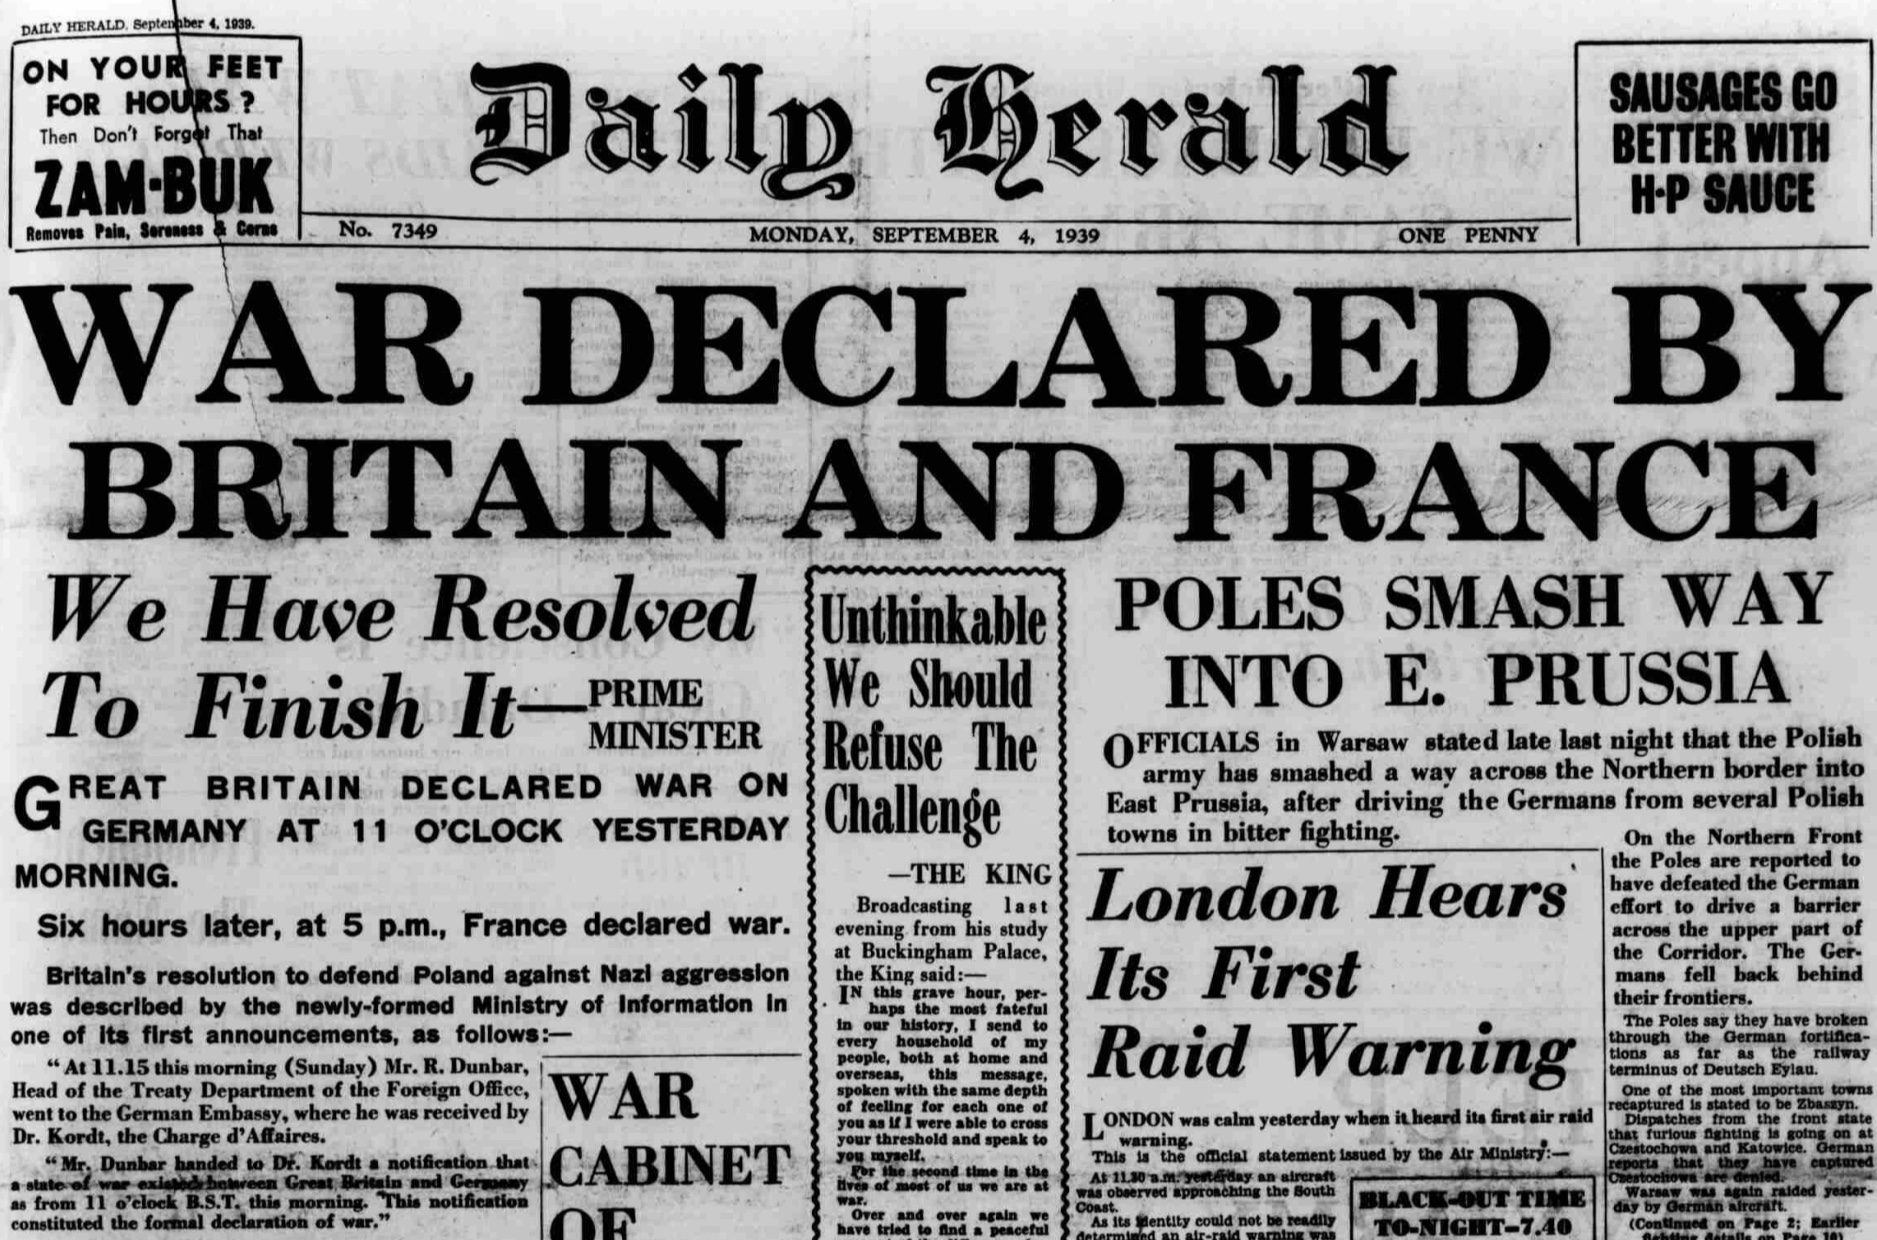
\includegraphics[width = \textwidth]{img/outbreak_wwii}

\end{frame}
% ----------------------------------------------------

% ----------------------------------------------------
\begin{frame}
\frametitle{What is international relations?}
\centering

\begin{itemize}
  \item Explaining \textbf{cooperation} and \textbf{conflict} between states
  \item Traditionally, focus on \textbf{war}
  \item Why war and not other phenomena?
\end{itemize}

\end{frame}
% ----------------------------------------------------

% ----------------------------------------------------
\begin{frame}
\frametitle{Other `topics' of IR}
\centering

\begin{itemize}[<+->]
  \item International Political Economy
  \item International Organizations
  \item Human Rights
  \item Development studies, foreign policy, ...
\end{itemize}

\end{frame}
% ----------------------------------------------------

% ----------------------------------------------------
\imageframe{img/wwi_declaration}
% ----------------------------------------------------


% ----------------------------------------------------
\begin{frame}
\frametitle{Why the focus on war?}
\centering

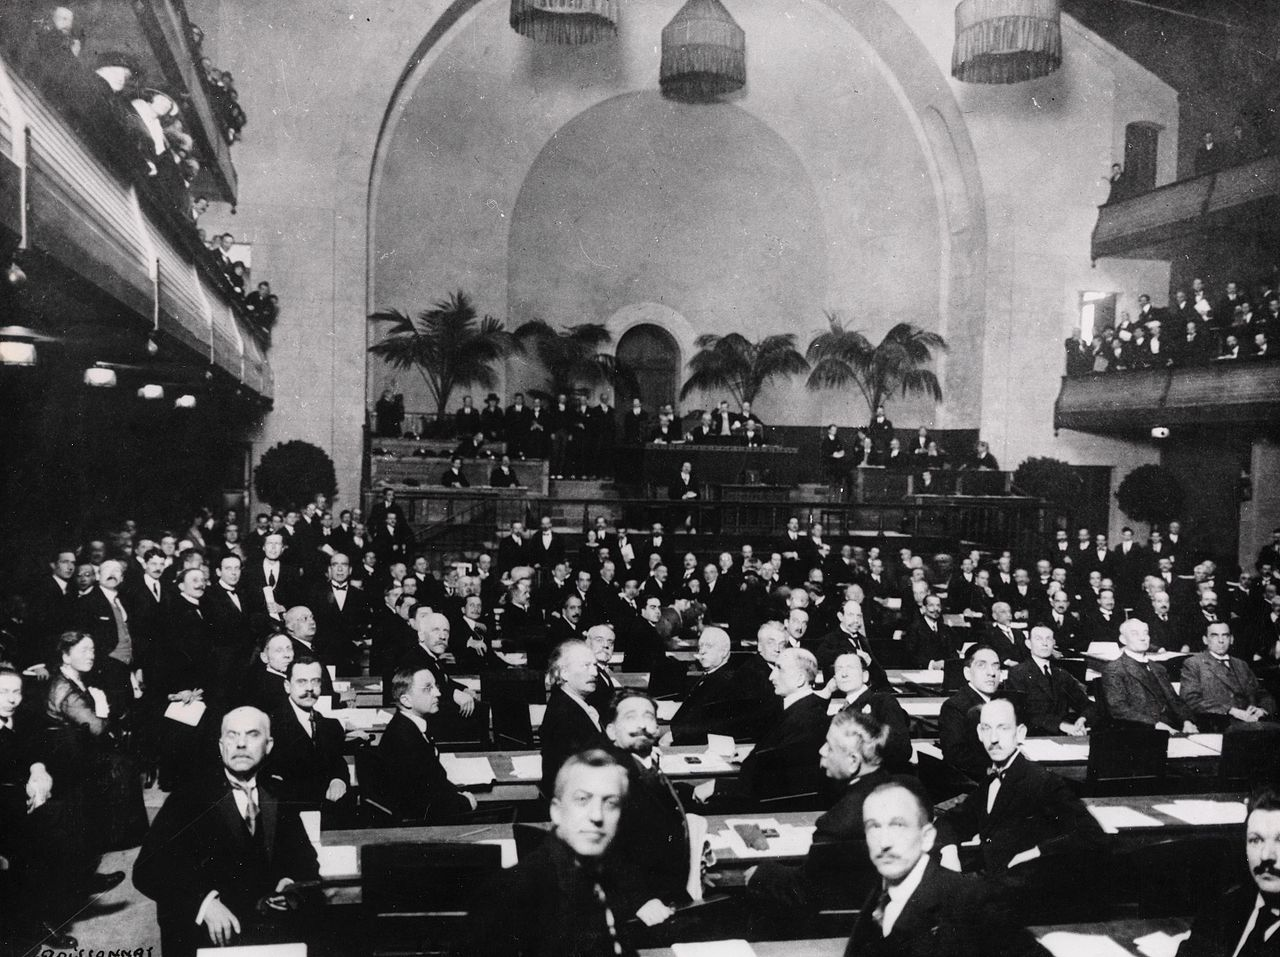
\includegraphics[width = 0.8\textwidth]{img/league_of_nations}

First meeting of the League of Nations, 1920

\end{frame}
% ----------------------------------------------------

% ----------------------------------------------------
\begin{frame}
\frametitle{How the war changed IR}
\centering

\begin{itemize}
  \item Efforts to achieve peace in Europe, role of Germany, etc
  \item IR before WWI: focus on colonianism and race, and on international law
  \item After the war, more interest and more funding for IR
  \begin{itemize}
    \item \textbf{1919}, Paris Peace Conference and the IR institute and the first IR dept in Aber
    \item Goal of IR: create peace after the Great War through the scientific study of the relationships between nations
  \end{itemize}
\end{itemize}

\end{frame}
% ----------------------------------------------------

% ----------------------------------------------------
\begin{frame}
\frametitle{How the war changed IR}
\centering

\begin{minipage}{0.49\textwidth}\centering
  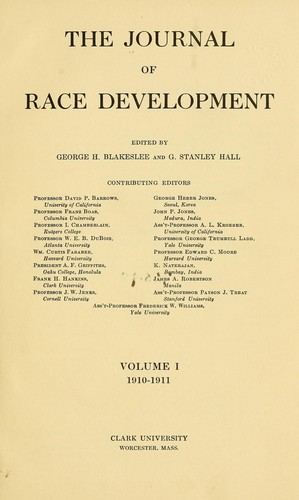
\includegraphics[width = 0.8\textwidth]{img/journal_race_dev}
\end{minipage}\hfill
\begin{minipage}{0.49\textwidth}\centering
  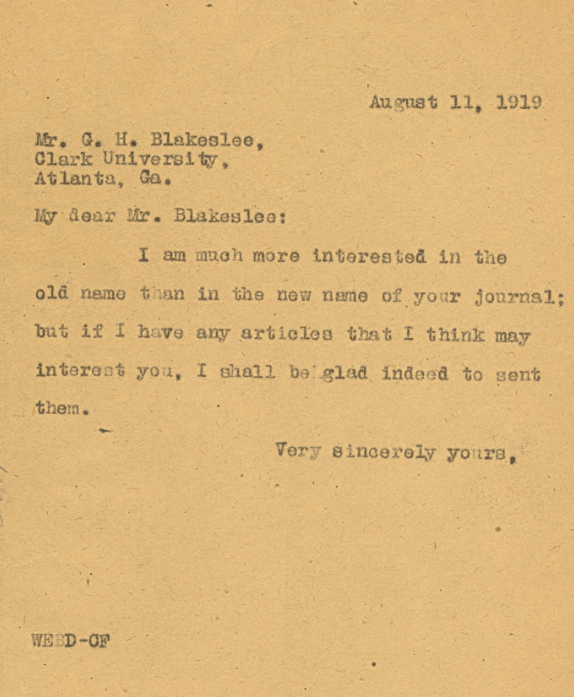
\includegraphics[width = 0.8\textwidth]{img/dubois_letter}\\{\small Letter by WEB DuBois after it changed its name (would later become \textit{Foreign Affairs})}
\end{minipage}

\end{frame}
% ----------------------------------------------------

% ----------------------------------------------------
\begin{frame}
\frametitle{War and IR}
\centering

\begin{minipage}{.49\textwidth}\centering
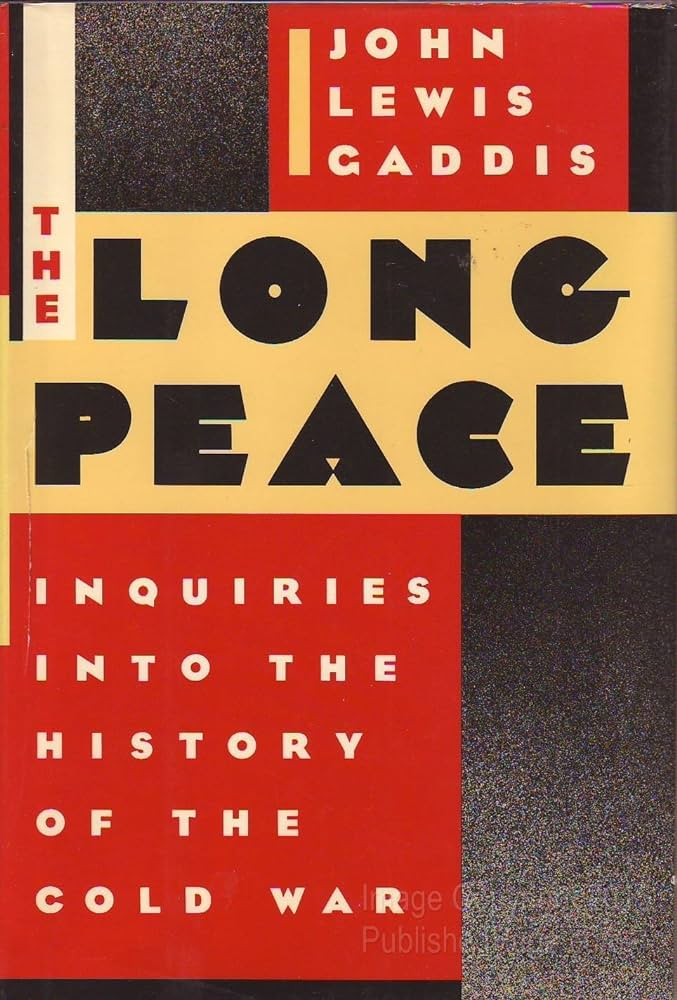
\includegraphics[width = 0.9\textwidth]{img/longpeace}
\end{minipage}\hfill
\begin{minipage}{.49\textwidth}\centering
\only<2>{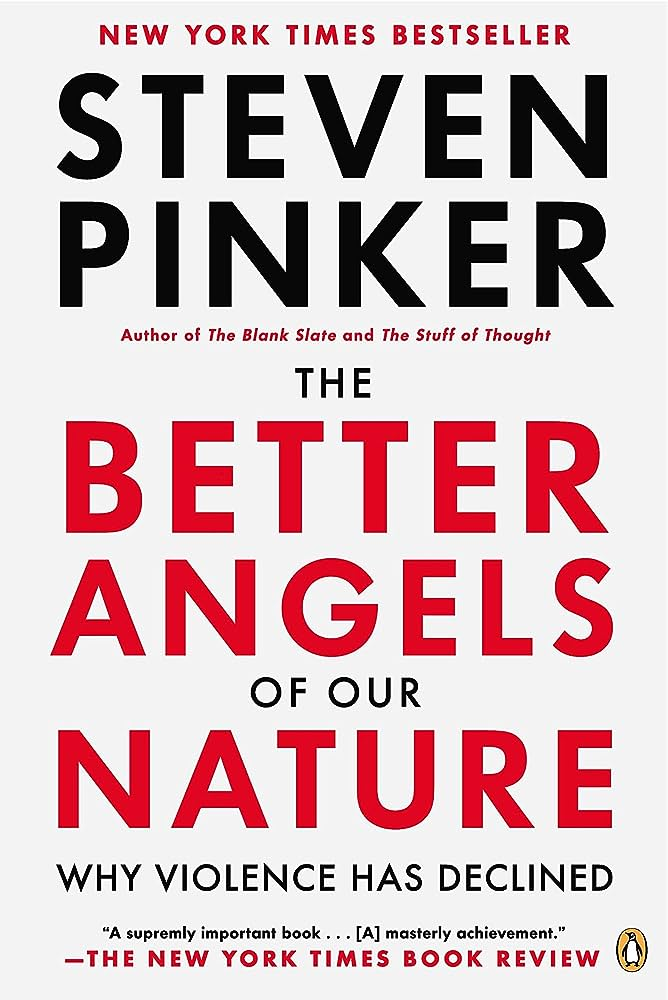
\includegraphics[width = 0.9\textwidth]{img/pinker}}
\end{minipage}

\end{frame}
% ----------------------------------------------------

% ----------------------------------------------------
\begin{frame}
\frametitle{War and IR}
\centering

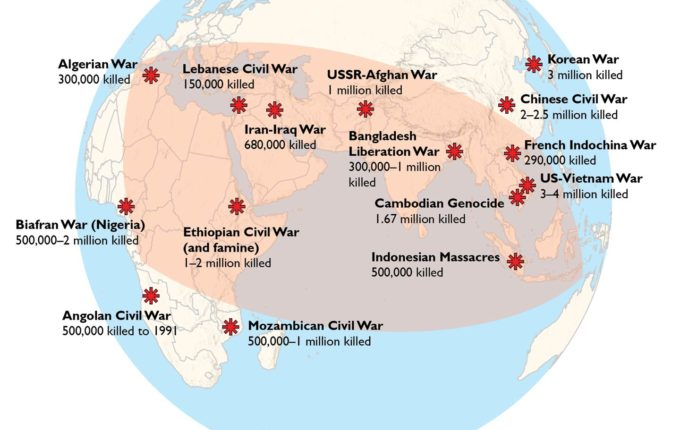
\includegraphics[width = \textwidth]{img/coldwar_conflicts}

\end{frame}
% ----------------------------------------------------

% ----------------------------------------------------
\begin{frame}
\frametitle{War and IR}
\centering

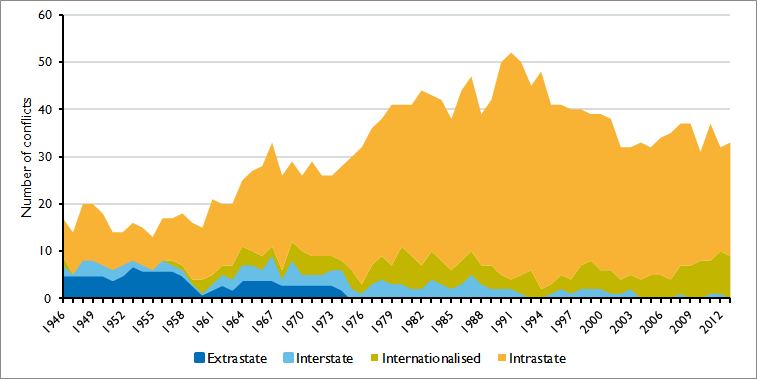
\includegraphics[width = \textwidth]{img/armed_conflicts}

\end{frame}
% ----------------------------------------------------

% ----------------------------------------------------
\begin{frame}
\frametitle{Main perspectives in IR}
\centering

\begin{itemize}
  \item<1-> \textbf{Realism}
  \item<1-> \textbf{Liberalism}
  \item<1-> \textbf{Constructivism}
  \item[]
  \item<2-> There are others: Marxism, feminism, rationalism, etc
  \item<3-> Again, usually applied to wars but can also explain many other things, e.g.
  \begin{itemize}
    \item European integration
    \item Spread of Human Rights
  \end{itemize}
  \item<3-> And actually some are better suited for this things
\end{itemize}

\end{frame}
% ----------------------------------------------------

% ----------------------------------------------------
\begin{frame}
\frametitle{Early realism}
\centering

\begin{itemize}
  \item \textbf{Human nature} is what explains international relations
  \begin{itemize}
    \item You have wars because humans are predisposed to fight wars, kind of
  \end{itemize}
  \item And the context is \textbf{power politics}
  \begin{itemize}
    \item Political actions are constrained by political and economic power and want to increase it
  \end{itemize}
  \item<2-> Classics: think Machiavelli's Prince (also Thucydides, Hobbes)
  \item<2-> More modern ones: E. H. Carr, Morgenthau (\textit{animus dominandi}), Niebuhr (\textit{sinful nature}), etc
\end{itemize}

\end{frame}
% ----------------------------------------------------

% ----------------------------------------------------
\begin{frame}
\frametitle{Early liberalism}
\centering

\begin{minipage}{.58\textwidth}\centering
\begin{itemize}
  \item Also called \textbf{liberal idealism}
  \item Basic idea is that war is \textbf{not inevitable} as long as liberal political principles are also present in the international system
  \item Explains the League of Nations, but also Wilson's Fourteen Points
  \begin{itemize}
    \item open int'l treaties, open trade, settle colonial struggles, association of nation-states...
  \end{itemize}
\end{itemize}
\end{minipage}\hfill
\begin{minipage}{.39\textwidth}\centering
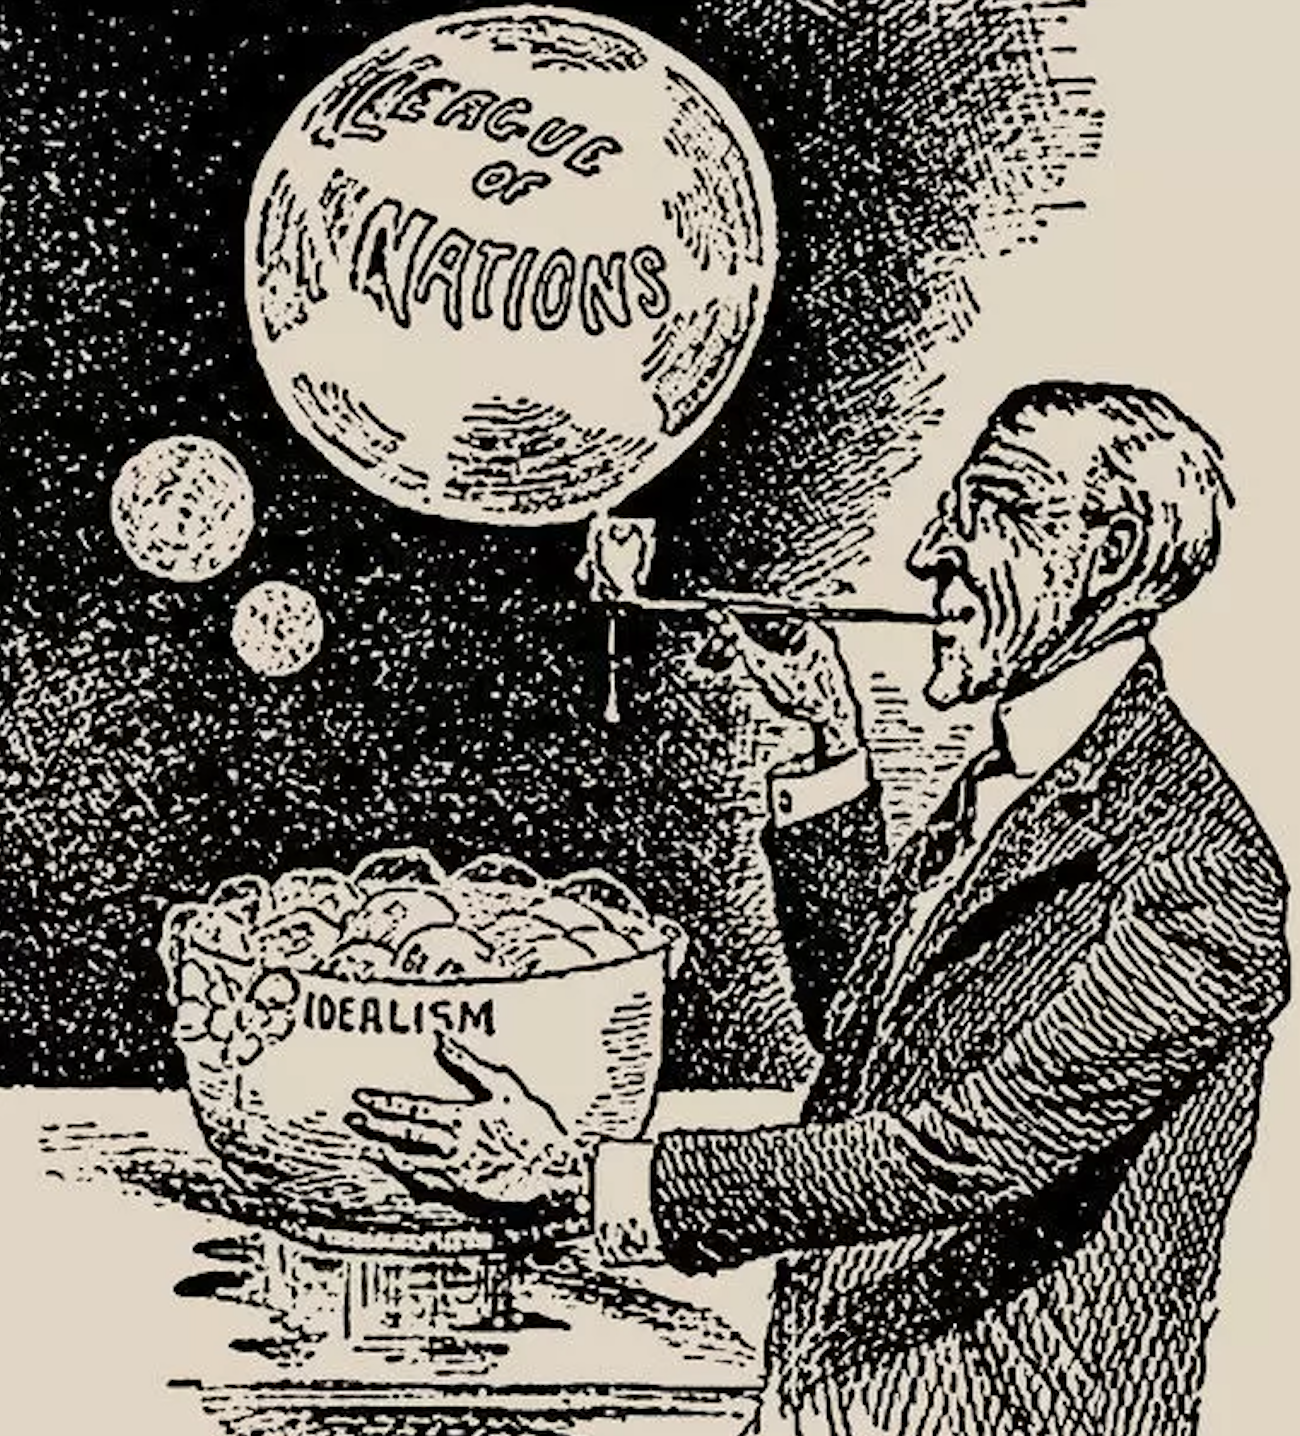
\includegraphics[width = \textwidth]{img/wwilson}\\{\small Woodrow Wilson}
\end{minipage}

\end{frame}
% ----------------------------------------------------


% ----------------------------------------------------
\begin{frame}
\frametitle{Waltz's neorealism (or structural neorealism)}
\centering


\begin{minipage}{0.71\textwidth}\centering
\begin{itemize}[<+->]
\item Understanding war through different levels of analyses (`images')
\item \textbf{First image: the man} (aka. individuals)
  \begin{itemize}
  \item Wars caused by the psychology of political leaders, or human nature (classical realism)
  \end{itemize}
\item \textbf{Second image: the state}
  \begin{itemize}
  \item Wars caused by the internal structure of a state (back then, Marxism)
  \end{itemize}
\item \BGyellow{\textbf{Third image:} \textbf{the international system}}
  \begin{itemize}
  \item War explained by the relationships between states: international anarchy
  \item Hobbesian view of the international system: no law, no constraints, no ``automatic harmony''
  \end{itemize}
% \item As a realist, he thought that the third image was the most influential one
\end{itemize}
\end{minipage}\hfill
\begin{minipage}{0.28\textwidth}\centering
\frame{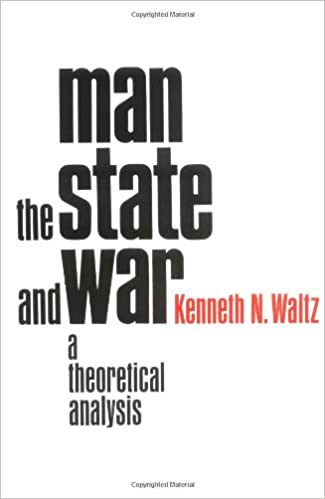
\includegraphics[width = 0.9\textwidth]{img/waltz}}\\
{\small Kenneth Waltz (1957)}
\end{minipage}

\end{frame}
% ----------------------------------------------------

% ----------------------------------------------------
\begin{frame}
\frametitle{Realism}
\centering

\begin{itemize}
\item<1-> Basic ideas behind structural realism:
  \begin{itemize}
  \item Main actors in world politics: sovereign states
  \item Context: international anarchy
  \item Goal of each state: security, power, wealth
  \end{itemize}
\item<2-> This perspective understands that war is explained by the \textit{distribution of power} at the international level
\item<3-> Wars break out because of predatory dynamics, conflict spirals (e.g. security dilemma), or pure preventive wars
\item<4-> `Defensive' (security) and `offensive' (power) realists
\end{itemize}

\end{frame}
% ----------------------------------------------------

% ----------------------------------------------------
\begin{frame}
\frametitle{Modern liberalism}
\centering

\begin{itemize}[<+->]
  \item It's not about the game, it's about the players
  \item Liberals do not accept the pessimism of realism: the international arena is not so Hobbesian, and states are able to cooperate and not fight each other constantly, etc
  \item \BGyellow{Institutional liberalism}: we need to foster cooperation through \textit{international organizations} and \textit{regime type} (or regime change)
  \item We'll see next the main arguments for war: democratic peace and capitalist peace
\end{itemize}

\end{frame}
% ----------------------------------------------------

% ----------------------------------------------------
\begin{frame}
\frametitle{Constructivism}
\centering

\begin{itemize}
  \item<1-> It's not only about material stuff, you have to pay attention to \textbf{ideology} (broadly defined)
  \item<2-> Leaders' self-perceived position and goals, identities, etc are socially constructed
  \item<2-> `Anarchy is what states make of it` (Alexander Wendt)
  \item<3-> Importance of \textbf{norms}
\end{itemize}

\end{frame}
% ----------------------------------------------------

% ----------------------------------------------------
\begin{frame}
\frametitle{Other approaches}
\centering

\begin{itemize}[<+->]
  \item We'll see some other perspectives applied the explanation of wars, but e.g.:
  \item \textbf{Marxism} does not focus on cooperation vs conflict but rather on how material incentives determine international relations (e.g. dependence theory and North-South relations)
  \item \textbf{Rationalism} emphasizes rational choice theory and its application to state's decisions (think of game theory)
  \item Others, such as \textbf{feminist} or \textbf{psychological} IR theories
\end{itemize}

\end{frame}
% ----------------------------------------------------

% ----------------------------------------------------
\imageframe{img/thucy}
% ----------------------------------------------------

% ----------------------------------------------------
\begin{frame}
\frametitle{European integration and consequences?}
\centering

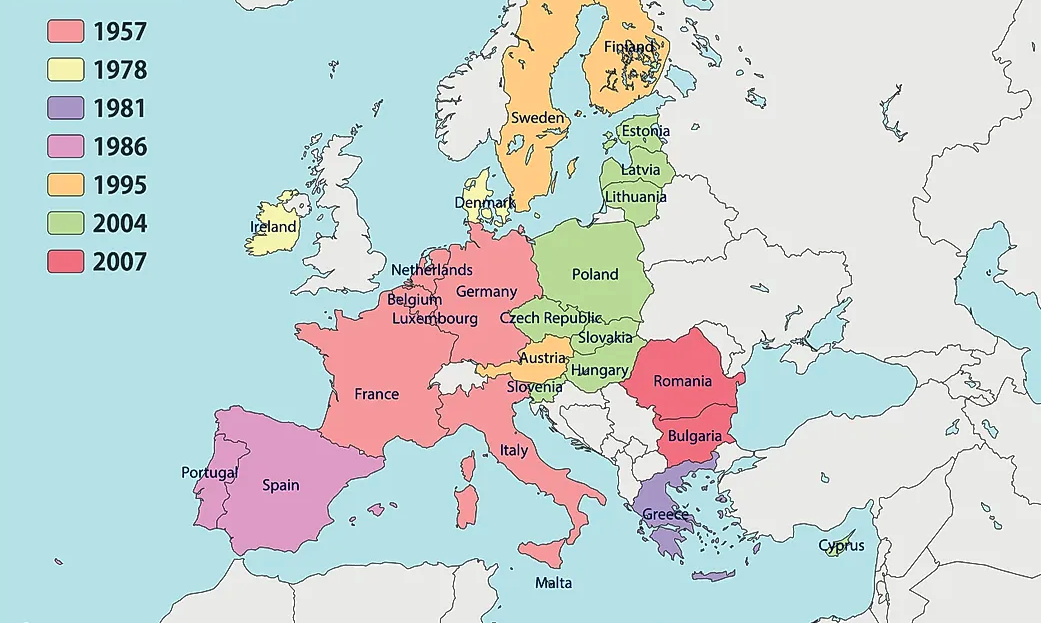
\includegraphics[width = \textwidth]{img/EU}

\end{frame}
% ----------------------------------------------------

% ----------------------------------------------------
\begin{frame}
\frametitle{International Human Rights?}
\centering

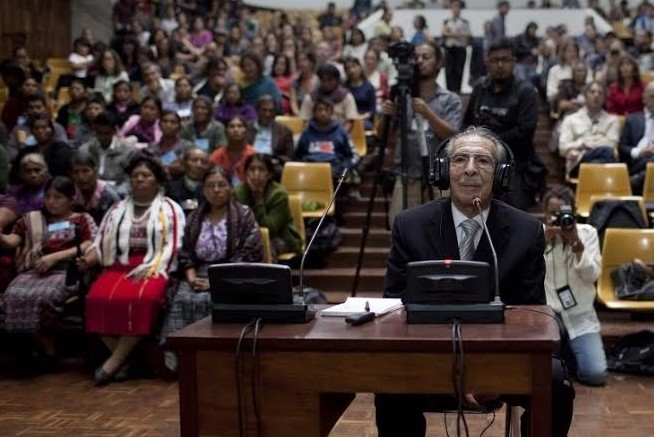
\includegraphics[width = 0.8\textwidth]{img/riosmontt}

{\small Ríos Montt during trial}

\end{frame}
% ----------------------------------------------------

% ----------------------------------------------------
\begin{frame}
\frametitle{Difference between IR and comparative politics}
\centering

\begin{itemize}
  \item Comparative politics and IR studying similar topics
  \item Just different perspectives, often overlapped
  \item Example of \textbf{democratization}
  \begin{itemize}
    \item \href{https://dartthrowingchimp.files.wordpress.com/2012/09/politymovie3.gif}{Evolution of Polity IV across time}
  \end{itemize}
  \item IR and different types of political violence
\end{itemize}

\end{frame}
% ----------------------------------------------------

% ----------------------------------------------------
\begin{frame}
\frametitle{Political violence more generally}
\centering

\begin{tabular}{m{1.75cm}|m{4cm}m{4cm}}
& {\color{gray}{\footnotesize Target:}} \newline State & {\color{gray}{\footnotesize Target:}} \newline Non-State \\\hline\\
{\color{gray}{\footnotesize Perpetrator:}} \newline State & Interstate war & State repression \newline Genocide \newline Ethnic cleansing \\\\
{\color{gray}{\footnotesize Perpetrator:}} \newline Non-State & Organized crime \newline Mass protests (rebellion) \newline Military coup \newline Political assassination* \newline Civil War \newline Terrorism & Intercommunal violence\\\\\hline
\end{tabular}

\end{frame}
% ----------------------------------------------------

\end{document}
